\paragraph{QuizziPedia::Front-End::ModelViews::QuestionnaireManagementModelView}
	
	\label{QuizziPedia::Front-End::ModelViews::QuestionnaireManagementModelView}
	
	\begin{figure}[ht]
		\centering
		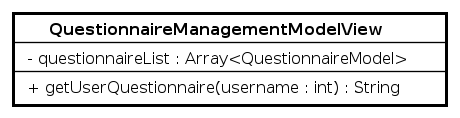
\includegraphics[scale=0.8,keepaspectratio]{UML/Classi/Front-End/QuizziPedia_Front-end_ModelView_QuestionnaireManagementModelView.png}
		\caption{QuizziPedia::Front-End::ModelViews::QuestionnaireManagementModelView}
	\end{figure} \FloatBarrier
	
	\begin{itemize}
		\item \textbf{Descrizione}: classe di tipo modelview la cui istanziazione è contenuta all'interno della variabile di ambiente \texttt{\$scope} di \textit{Angular\ped{G}}. All'interno di essa sono presenti le variabili e i metodi necessari per il \textit{Two-Way Data-Binding\ped{G}} tra la \textit{view\ped{G}} \texttt{QuestionnaireManagementView} e il \textit{controller\ped{G}} \texttt{QuestionnaireManagementController};
		\item \textbf{Utilizzo}: viene utilizzata per effettuare il \textit{Two-Way Data-Binding\ped{G}} tra la \textit{view\ped{G}} \texttt{QuestionnaireManagementView} e il \textit{controller\ped{G}} \texttt{QuestionnaireManagementController} rendendo disponibili variabili e metodi;
		\item \textbf{Relazioni con altre classi}: 
		\begin{itemize}
			\item \textbf{IN \texttt{QuestionnaireManagementView}}: \textit{view\ped{G}} principale per la gestione dei questionari; 
			\item \textbf{IN \texttt{QuestionnaireManagementController}}: questa classe permette di gestire tutti i questionari creati da un utente;
		\end{itemize}
		\item \textbf{Attributi}: 
		\begin{itemize}
			\item \texttt{- questionnaireList: Array} \\ \texttt{array} contenente la lista dei questionari creati; ogni questionario sarà rappresentato come un oggetto.
		\end{itemize}
		\item \textbf{Metodi}:
		\begin{itemize}
				\item \texttt{+ getUserQuestionnaire(username: String) QuestionnaireModel[]}: \\Metodo che ritorna tutti i questionari creati da un utente in un array di QuestionnaireModel.
				\textbf{Parametri}:
				\begin{itemize}
					\item \texttt{username: String}\\ 
					Parametro che indica l'identificativo dell'utente del quale vogliamo scaricare tutti i questionari.
				\end{itemize}
		\end{itemize} 
	\end{itemize}
	
	